\chapter{Vizualizacija podatkov}

\section{Knjižnica Matplotlib in njena namestitev}
Za vizualizacijo podatkov bomo uporabljali knjižnico Matplotlib, ki predstavlja osnovo za risanje kakršnihkoli grafov. Ker v osnovni različici jezika Python še ni nameščen, ga moramo pred uporabo namestiti (če imate nameščeno distribucijo Anaconda, imate to knjižnico že nameščeno). Kot smo spoznali v poglavju \ref{ch:moduli} lahko za namestitev knjižnice uporabimo orodje \texttt{pip}, tako da zaženemo ukazno vrstico svojega operacijskega sistema (ne okolja IDLE) in vanjo vpišemo
\begin{lstlisting}[language=bash]
> pip install matplotlib
\end{lstlisting}
Podrobnejša navodila za namestitev paketov smo podali že v poglavju \ref{ch:moduli}, zato jih tu ne bomo podvajali. Če ima vaš računalnik povezavo z internetom, bo orodje \texttt{pip} samo preneslo potrebne namestitvene datoteke in knjižnico namestilo.

Za vizualizacijo naših podatkov bomo uporabili Matplotlibov vmesnik \angl{interface} \texttt{pyplot}, ki nam risanje precej olajša. V svoje programe ga bomo uvozili takole:
\begin{lstlisting}[language=Python, showstringspaces=false]
import matplotlib.pyplot as plt
\end{lstlisting}
Zdaj lahko do funkcij za risanje grafov dostopamo takole:
\begin{lstlisting}[language=Python, showstringspaces=false]
plt.ime_funkcije(argumenti)
\end{lstlisting}

\section{Funkciji \texttt{plot} in \texttt{show}}

Začeli bomo s funkcijo \texttt{plot}, ki omogoča izris črtnega grafa \angl{line plot}. V osnovi ji lahko podamo zgolj en seznam. Poskusimo:
\begin{lstlisting}[language=Python]
>>> Y = [1, 3, 9, 12]
>>> plt.plot(Y)
[<matplotlib.lines.Line2D object at 0x000001DD7FB28860>]
\end{lstlisting}
Nekaj se je očitno zgodilo, grafa pa še vedno ne vidimo. Funkcija \texttt{plot} deluje tako, da grafe riše v ozadju in te dodaja na risalno površino, ki pa jo pokaže, šele ko pokličemo funkcijo \texttt{show}.
\begin{lstlisting}[language=Python, showstringspaces=false]
>>> plt.show()
\end{lstlisting}
Zdaj se je prikazal graf, ki ga prikazuje slika \ref{img:plt1}.
\begin{figure}
    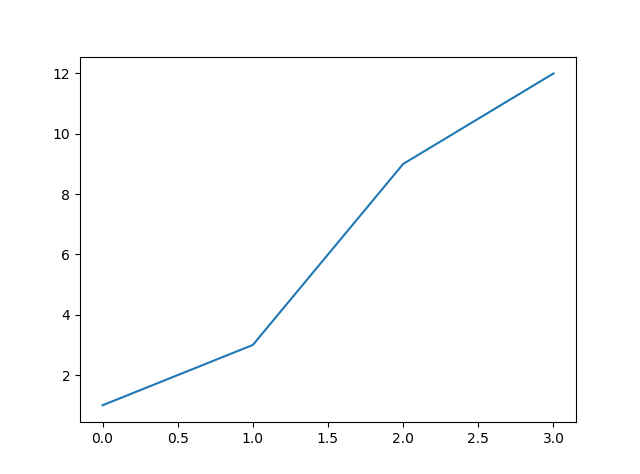
\includegraphics[width=\linewidth]{img/plt1.png}
    \caption{Črtni graf, pri čemer smo podali koordinate točk na osi $y$.}
    \label{img:plt1}
\end{figure}
Točke, ki smo jih podali funkciji \texttt{plot}, očitno predstavljajo koordinate $y$ narisanega grafa. Točke na osi $x$ je Matplotlib določil kar glede na indekse točke v seznamu \texttt{Y}. To lahko spremenimo, tako da funkcijo \texttt{plot} pokličemo z dvema seznamoma, pri čemer prvi določa koordinate točk na osi $x$ drugi pa koordinate točk na osi $y$\footnote{To se zgodi v primeru, ko imamo v prvem seznamu številske vrednosti. Če bi imeli v prvem seznamu nize, bi bili ti uporabljeni kot oznake na osi $x$, pri čemer bi bile lokacije točk na osi $x$ zopet določene kar z indeksi točk na osi $y$.}. Seznama morata biti seveda enakih dolžin. Do enakega grafa kot zgoraj, bi lahko prišli takole: 
\begin{lstlisting}[language=Python, showstringspaces=false]
>>> Y = [1, 3, 9, 12]
>>> X = range(len(Y))
>>> plt.plot(X, Y)
[<matplotlib.lines.Line2D object at 0x000002042BEBC128>]
plt.show()
\end{lstlisting}
Os $x$ bi lahko tudi spremenili. Poskusimo:
\begin{lstlisting}[language=Python, showstringspaces=false]
>>> X = [1,3,4,5]
>>> Y = [1, 3, 9, 12]
>>> plt.plot(X,Y)
[<matplotlib.lines.Line2D object at 0x000002042A9D0DA0>]
>>> plt.show()
\end{lstlisting}
Graf, ki smo ga narisali tako, prikazuje slika \ref{img:plt2}.
\begin{figure}
    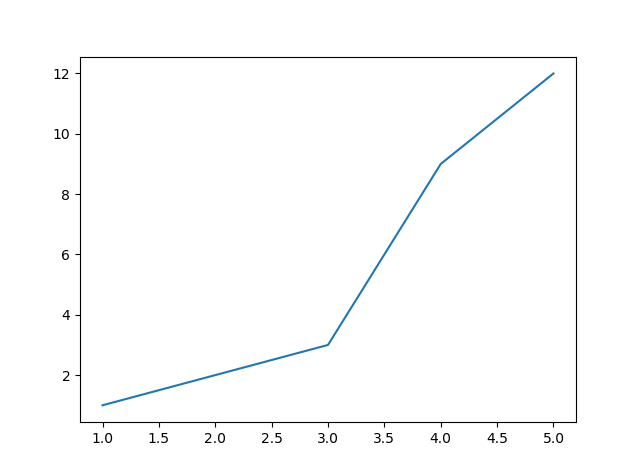
\includegraphics[width=\linewidth]{img/plt2.png}
    \caption{Črtni graf, pri čemer smo podali koordinate točk na obeh oseh.}
    \label{img:plt2}
\end{figure}
Na sliki je prikazan samo zadnji graf. Kam je izginil prejšnji? Kot smo že omenili knjižnica Matplotlib grafe riše na risalni površini v ozadju. Te prikaže, ko pokličemo funkcijo \texttt{show}, hkrati pa takrat risalno površino tudi počisti. Če hočemo na isti sliki prikazati več grafov, bomo pred klicanjem funkcije \texttt{show} narisali več grafov. Poskusimo to kar na zgledu s plačami, in sicer bi radi narisali podatke o povprečnih bruto plačah. Predpostavljali bomo, da smo funkcijo \texttt{uvozi\_place} shranili v program \texttt{place\_beri.py} in da se ta program nahaja v naši trenutni delovni mapi. Najprej bomo uvozili funkcijo za uvoz podatkov o plačah zraven pa še knjižnico Matplotlib:
\begin{lstlisting}[language=Python, showstringspaces=false]
>>> from place_beri import uvozi_place
>>> import matplotlib.pyplot as plt
\end{lstlisting}
Potem preberimo podatke o plačah:
\begin{lstlisting}[language=Python]
>>> place = uvozi_place('place.csv')
\end{lstlisting}
in potegnemo sezname is slovarjev:
\begin{lstlisting}[language=Python]
>>> MJ = place['Javni sektor']['mesec']
>>> ZJ = place['Javni sektor']['bruto']
>>> MZ = place['Zasebni sektor']['mesec']
>>> ZZ = place['Zasebni sektor']['bruto']
\end{lstlisting}
Zdaj bomo kot koordinate na osi $x$ podali podatke o mesecih. Tako se nam bodo na osi $x$ izpisali kar podatki o mesecih. Kot koordinate na osi $y$ podamo podatke o zneskih. Potem bomo poklicali še funkcijo za prikaz grafa.
\begin{lstlisting}[language=Python, showstringspaces=false]
>>> plt.plot(MJ, ZJ)
>>> plt.plot(MZ, ZZ)
>>> plt.show()
\end{lstlisting}
Več grafov lahko na isto sliko narišemo tudi tako, da naštejemo pare seznamov kar po vrsti. Takole: 
\begin{lstlisting}[language=Python, showstringspaces=false]
>>> plt.plot(MJ, ZJ, MZ, ZZ)
>>> plt.show()
\end{lstlisting}
Kljub temu, da je rezultat v zgornjih dveh primerih enak, bomo raje uporabljali prvi način.
Zapišimo zdaj vse skupaj kot program \texttt{risi\_place.py}.
\begin{lstlisting}[language=Python,numbers=left]
from place_beri import uvozi_place # funkcija za uvoz
import matplotlib.pyplot as plt 

# uvozi podatke v slovar
place = uvozi_place('place.csv')
# pridobi sezname iz slovarja
MJ = place['Javni sektor']['mesec']
ZJ = place['Javni sektor']['bruto']
MZ = place['Zasebni sektor']['mesec']
ZZ = place['Zasebni sektor']['bruto']

plt.plot(MJ, ZJ) # riši javni sektor
plt.plot(MZ, ZZ) # riši zasebni sektor
plt.show() # prikaži graf
\end{lstlisting}
Rezultat izvedbe zgornjega programa prikazuje slika \ref{img:plt3}.
\begin{figure}
    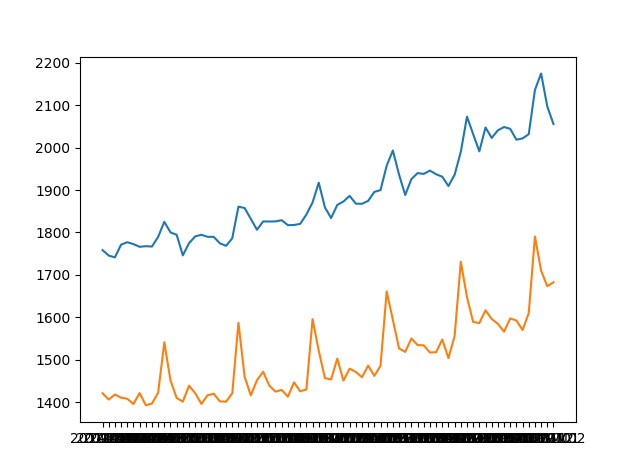
\includegraphics[width=\linewidth]{img/plt3.png}
    \caption{Osnovni izris podatkov o plačah.}
    \label{img:plt3}
\end{figure}

\section{Dodajanje oznak}
Vsak graf seveda potrebuje oznake. Označiti moramo kaj prikazuje posamezna os, za kar lahko uporabimo funkciji \texttt{xlabel} in \texttt{ylabel}, ki kot argument prejmeta niz, ki ga želimo prikazati. V našem primeru bi bilo smiselno napisati takole:
\begin{lstlisting}[language=Python]
plt.xlabel("mesec")
plt.ylabel("znesek [EUR]")
\end{lstlisting}
Dodamo lahko tudi naslov grafa z uporabo funkcije \texttt{title}. Takole:
\begin{lstlisting}[language=Python]
plt.title("Povprečne mesečne plače")
\end{lstlisting}

Manjka seveda tudi legenda. Kaj prikazuje modra linija in kaj oranžna? Legendo lahko dodamo tako, da oznake dodamo posameznemu grafu kar med izrisom. Funkciji \texttt{plot} lahko preko opcijskega argumenta \texttt{label} podamo niz, ki predstavlja oznako grafa, ki ga bo izrisala. V našem primeru bi to naredili takole:
\begin{lstlisting}[language=Python]
plt.plot(MJ, ZJ, label='Javni sektor') # riši javni sektor
plt.plot(MZ, ZZ, label='Zasebni sektor') # riši zasebni sektor
\end{lstlisting}
Če želimo legendo pokazati, moramo poklicati še funkcijo \texttt{legend}, ki prikaz legende vklopi:
\begin{lstlisting}[language=Python]
plt.legend()
\end{lstlisting}
Vsebino legende, ki jo želimo izpisati bi lahko podali tudi neposredno funkciji \texttt{legend}. Takole:
\begin{lstlisting}[language=Python]
plt.legend(['Javni sektor', 'Zasebni sektor'])
\end{lstlisting}
Pri tem moramo paziti na to, da oznake v legendi podajamo v enakem vrstnem redu, kot smo izvajali risanje grafov.


Zapišimo celoten program, ga poženimo in poglejmo rezultat. 
\begin{lstlisting}[language=Python,numbers=left]
from place_beri import uvozi_place # funkcija za uvoz
import matplotlib.pyplot as plt

# uvozi podatke v slovar
place = uvozi_place('place.csv')
# pridobi sezname iz slovarja
MJ = place['Javni sektor']['mesec']
ZJ = place['Javni sektor']['bruto']
MZ = place['Zasebni sektor']['mesec']
ZZ = place['Zasebni sektor']['bruto']

plt.plot(MJ, ZJ) # riši javni sektor
plt.plot(MZ, ZZ) # riši zasebni sektor

# dodaj oznake
plt.xlabel("mesec")
plt.ylabel("znesek [EUR]")
plt.title("Povprečne mesečne plače")
plt.legend(['Javni sektor', 'Zasebni sektor'])

plt.show() # prikaži graf
\end{lstlisting}
Rezultat izvedbe zgornjega programa prikazuje slika \ref{img:plt4}.
\begin{figure}
    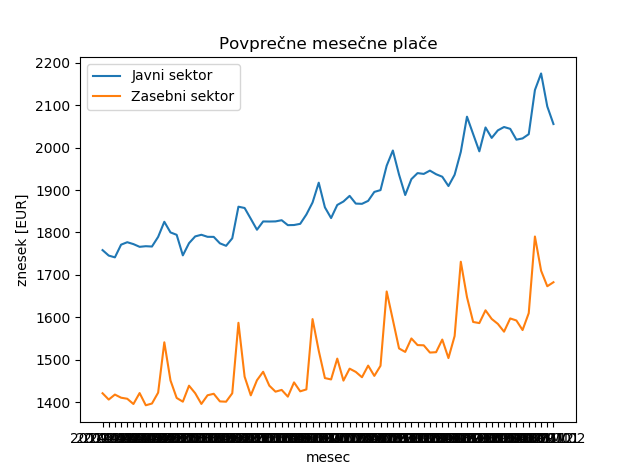
\includegraphics[width=\linewidth]{img/plt4.png}
    \caption{Izris podatkov o plačah z dodanimi oznakami.}
    \label{img:plt4}
\end{figure}

\section{Še malo prilagajanja oznak}
Kar nam še vedno ni všeč na sliki \ref{img:plt4}, je neberljiv izpis na osi $x$. Če graf približamo, vidimo, da je na oseh izpisan podatek o mesecu. Mogoče bi bilo bolje, če bi ta podatek izpisali samo vsak januar, poleg tega pa bi bilo potem smiselno izpisati samo informacijo o letu (brez meseca). Poskusimo odrezati rezino po mesecih od začetka do konca, pri čemer za korak nastavimo vrednost 12.
\begin{lstlisting}[language=Python, showstringspaces=false]
>>> MJ[::12]
['2014M01', '2015M01', '2016M01', '2017M01', '2018M01',
'2019M01', '2020M01']
\end{lstlisting}
Pripravimo si seznam \texttt{oznake}, ki bo vseboval samo podatke o letih. Vzeli bomo vsak 12-ti podatek iz obstoječega seznama mesecev (izhajamo lahko bodisi iz seznama \texttt{MJ} ali \texttt{MZ}), pri čemer bomo upoštevali samo prve štiri znake (podatek o letu). 
\begin{lstlisting}[language=Python, showstringspaces=false]
oznake = []
for mj in MJ[::12]: # vzamemo vsako 12-to oznako
    oznake.append(mj[:4]) # vzamemo samo podatek o letu
\end{lstlisting}
Določiti moramo še lokacije, kjer bomo te oznake prikazali. Trenutno so oznake prikazane na lokacijah, ki se ujemajo z njihovimi indeksi, torej bi lahko lokacije oznak dobili s seznamoma \texttt{range(len(MJ))} ter \texttt{range(len(MZ))}. Ker bi radi prikazali vsako 12-to oznako, bomo morali torej upoštevati tudi vsako 12-to lokacijo. Takole:
\begin{lstlisting}[language=Python, showstringspaces=false]
# vsaka 12-ta lokacija
lokacije = range(0, len(MJ), 12) 
\end{lstlisting}

Lokacijo in vsebino oznak lahko zdaj našemu risarju podamo preko funkcije \texttt{xticks} (če bi želeli prilagajati oznake na osi $y$, bi uporabili funkcijo \texttt{yticks}):
\begin{lstlisting}[language=Python, showstringspaces=false]
plt.xticks(lokacije, oznake)
\end{lstlisting}

Celoten program je zdaj sledeč:
\begin{lstlisting}[language=Python, showstringspaces=false,numbers=left]
from place_beri import uvozi_place # funkcija za uvoz
import matplotlib.pyplot as plt

# uvozi podatke v slovar
place = uvozi_place('place.csv')
# pridobi sezname iz slovarja
MJ = place['Javni sektor']['mesec']
ZJ = place['Javni sektor']['bruto']
MZ = place['Zasebni sektor']['mesec']
ZZ = place['Zasebni sektor']['bruto']


# dodaj oznake
plt.xlabel("leto") # zdaj prikazujemo samo leta
plt.ylabel("znesek [EUR]")
plt.title("Povprečne mesečne plače")
plt.legend(['Javni sektor', 'Zasebni sektor'])

oznake = []
for mj in MJ[::12]: # vzamemo vsako 12-to oznako
    oznake.append(mj[:4]) # vzamemo samo podatek o letu

# vsaka 12-ta lokacija
lokacije = range(0, len(MJ), 12) 

plt.xticks(lokacije, oznake)

plt.show() # prikaži graf
\end{lstlisting}
Rezultat izvedbe programa prikazuje slika \ref{img:plt5}.
\begin{figure}
    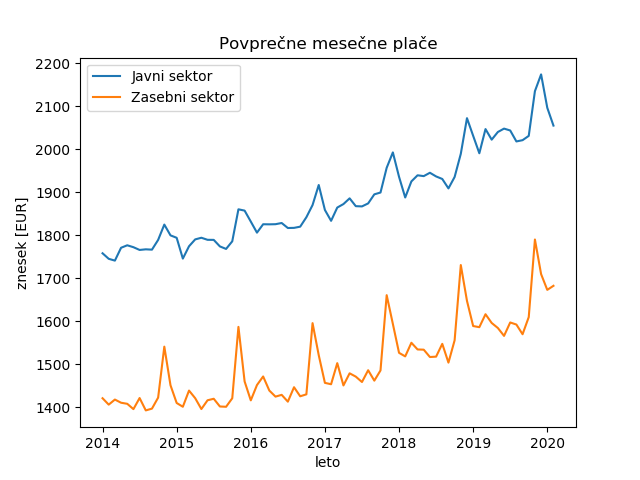
\includegraphics[width=\linewidth]{img/plt5.png}
    \caption{Izris podatkov o plačah s prilagojenimi oznakami na osi $x$. Namesto podatkov o mesecu smo izpisali podatke o letu.}
    \label{img:plt5}
\end{figure}

Kaj pa če bi imeli v podatkih o plačah še kakšen sektor več? Ker imamo podatke shranjene v dokaj prilagodljivi strukturi (slovarju), bi lahko izris naredili neodvisno od števila sektorjev. Enostavno se sprehodimo čez ključe slovarja in rišemo. Takole:
\begin{lstlisting}[language=Python]
for sektor in place:
    mesec = place[sektor]['mesec']
    znesek = place[sektor]['bruto']
    plt.plot(mesec, znesek, label=sektor)
\end{lstlisting}
Tokrat smo oznake grafov dodajali že kar med izrisovanjem preko argumenta \texttt{label}. Pri risanju oznak na osi $x$ lahko uporabimo kar spremenljivko \texttt{mesec}, v kateri so ostali podatki zadnjega sektorja (po sprehodu z zanko \texttt{for}). Celotna koda je sledeča: 
\begin{lstlisting}[language=Python, showstringspaces=false,numbers=left]
from place_beri import uvozi_place # funkcija za uvoz
import matplotlib.pyplot as plt

# uvozi podatke v slovar
place = uvozi_place('place.csv')
# pridobi sezname iz slovarja
MJ = place['Javni sektor']['mesec']
ZJ = place['Javni sektor']['bruto']
MZ = place['Zasebni sektor']['mesec']
ZZ = place['Zasebni sektor']['bruto']


plt.plot(MJ, ZJ) # riši javni sektor
plt.plot(MZ, ZZ) # riši zasebni sektor

# dodaj oznake
plt.xlabel("mesec")
plt.ylabel("znesek [EUR]")
plt.title("Povprečne mesečne plače")
plt.legend(['Javni sektor', 'Zasebni sektor'])

oznake = []
for mj in MJ[::12]: # vzamemo vsako 12-to oznako
    oznake.append(mj[:4]) # vzamemo samo podatek o letu

# vsaka 12-ta lokacija
lokacije = range(0, len(MJ), 12) 

# prikaži oznake na osi x
plt.xticks(lokacije, oznake)

plt.show() # prikaži graf
\end{lstlisting}

\section{Ostale prilagoditve izrisa}
Če nam grafi še vedno niso všeč, se lahko igramo naprej. Preko funkcije \texttt{plot} lahko nastavljamo barvo izrisa (argument \texttt{color}), debelino črte (argument \texttt{linewidth}), tip črte (argument \texttt{linestyle}) in še marsikaj. Poleg tega lahko določamo razpon osi (funkcija \texttt{axis}), rišemo več podgrafov (funkcija \texttt{subplot}) in graf shranjujemo v datoteko (funkcija \texttt{savefig}). Možnosti je res veliko in jih tukaj ne bomo več naštevali. Primere različnih grafov, ki jih lahko izrišemo z uporabo knjižnice Matplotlib, si lahko bralec pogleda (in prosto dostopno kodo prilagodi za risanje svojih grafov) na povezavi \url{https://matplotlib.org/gallery}.

\section{Ostali tipi grafov}

Matplotlib poleg črtnega diagrama (funkcija \texttt{plot}) omogoča risanje tudi ostalih tipov grafov, npr. stolpčnega diagrama \angl{bar plot} s funkcijo \texttt{bar}, histograma s funkcijo \texttt{hist}, kvartilnega diagrama s funkcijo \texttt{box} itd. Poglejmo si še primer izrisa stolpčnega diagrama, pri čemer bomo prikazali podatke o povprečnih plačah za leto 2018. Najprej iz podatkov izluščimo zgolj podatke za leto 2018. Hkrati se bomo morali sprehajati čez mesece in zneske. Ker sta seznama poravnana (isti indeks se nanaša na isti mesec), lahko naredimo sprehod s pomočjo funkcije \texttt{zip}. Znotraj sprehoda pogledamo, če se mesec nanaša na leto 2018 in v tem primeru mesec in znesek dodamo v nova seznama, ki se nanašata na leto 2018. To naredimo za javni in zasebni sektor posebej:
\begin{lstlisting}[language=Python, showstringspaces=false]
# uvozi podatke v slovar
place = uvozi_place('place.csv')
# pridobi sezname iz slovarja
MJ = place['Javni sektor']['mesec']
ZJ = place['Javni sektor']['bruto']
MZ = place['Zasebni sektor']['mesec']
ZZ = place['Zasebni sektor']['bruto']

MJ_2018 = []
ZJ_2018 = []
MZ_2018 = []
ZZ_2018 = []

for mj, zj in zip(MJ, ZJ):
    if "2018" in mj:
        MJ_2018.append(mj)
        ZJ_2018.append(zj)

for mz, zz in zip(MZ, ZZ):
    if "2018" in mz:
        MZ_2018.append(mz)
        ZZ_2018.append(zz)
\end{lstlisting}

Zdaj lahko podatke narišemo, pri čemer bomo za izris uporabili funkcijo \texttt{bar}. Ena izmed razlik med funkcijo \texttt{plot} in \texttt{bar} je, da moramo pri slednji lokacije stolpcev na osi $x$ vedno podati. Uporabimo lahko kar funkcijo \texttt{range}:
\begin{lstlisting}[language=Python, showstringspaces=false]
plt.bar(range(len(ZJ_2018)), ZJ_2018)
plt.bar(range(len(ZZ_2018)), ZZ_2018)
\end{lstlisting}

Z uporabo funkcije \texttt{xticks} lahko določimo še oznake na osi $x$:
\begin{lstlisting}[language=Python]
plt.xticks(range(len(MJ)), MJ)
\end{lstlisting}

Poglejmo si rezultat
\begin{lstlisting}[language=Python]
plt.show()
\end{lstlisting}
Prikazuje ga slika \ref{img:plt6}.
\begin{figure}
    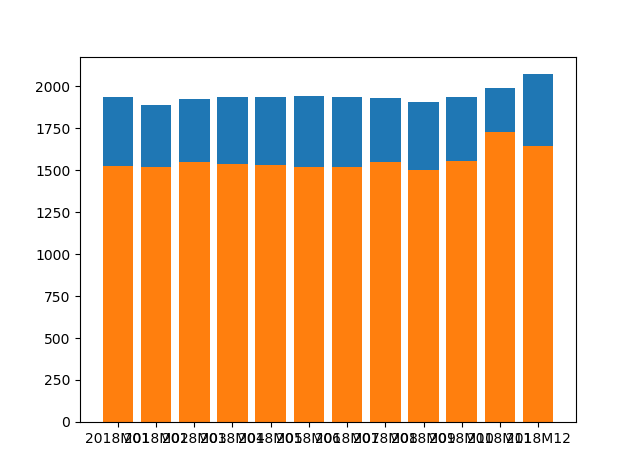
\includegraphics[width=\linewidth]{img/plt6.png}
    \caption{Izris podatkov o plačah za leto 2018 s stolpčnim diagramom.}
    \label{img:plt6}
\end{figure}
Oznake na osi $x$ so zopet moteče. Grafu bi lahko dodali naslov, da gre za leto 2018, na osi $x$ pa prikazali samo informacijo o mesecu. Tako bo postal graf bolj pregleden. Najprej iz oznak odstranimo podatek o letu. To lahko naredimo že med filtiranjem podatkov za leto 2018, kjer namesto stavkov \texttt{MJ\_2018.append(mj)} in \texttt{MZ\_2018.append(mz)} uporabimo stavka \texttt{MJ\_2018.append(mj[-3:])} in \texttt{MZ\_2018.append(mz[-3:])}. Naslov grafa dodamo s sledečo vrstico:
\begin{lstlisting}[language=Python]
plt.title('Podatki o plačah za leto 2018')
\end{lstlisting}
Dodajmo še legendo:
\begin{lstlisting}[language=Python, showstringspaces=false]
plt.legend(['Javni sektor', 'Zasebni sektor'])
\end{lstlisting}

Kar nas še moti je to, da sta grafa \emph{naložena} drug na drugega. Če bi npr. najprej izrisali zasebni sektor, bi ga javni sektor prekril. Bolj pravilno bi bilo, če bi grafa narisala drug ob drugemu. Kako lahko to naredimo? Tako, da en graf zamaknemo v levo, drugega pa v desno. Popravili bomo tudi širino stolpcev, da bodo malo ožji. Najprej določimo lokacije stolpcev:
\begin{lstlisting}[language=Python]
loc1 = list(range(len(ZJ_2018)))
loc2 = list(range(len(ZZ_2018)))
for i in range(len(loc1)):
    loc1[i] -= 0.2
    loc2[i] += 0.2
\end{lstlisting}
Zdaj te lokacije upoštevajmo pri izrisu, poleg tega pa preko izbirnega argumenta \texttt{width} nastavimo še širino stolpcev:
\begin{lstlisting}[language=Python]
plt.bar(loc1, ZJ_2018, width = 0.4)
plt.bar(loc2, ZZ_2018, width = 0.4)
\end{lstlisting}

Celoten program je zdaj sledeč:
\begin{lstlisting}[language=Python,numbers=left]
from place_beri import uvozi_place # funkcija za uvoz
import matplotlib.pyplot as plt

# uvozi podatke v slovar
place = uvozi_place('place.csv')
# pridobi sezname iz slovarja
MJ = place['Javni sektor']['mesec']
ZJ = place['Javni sektor']['bruto']
MZ = place['Zasebni sektor']['mesec']
ZZ = place['Zasebni sektor']['bruto']

# izluščimo podatke za leto 2018
MJ_2018 = []
ZJ_2018 = []
MZ_2018 = []
ZZ_2018 = []

for mj, zj in zip(MJ, ZJ):
    if "2018" in mj:
        MJ_2018.append(mj[-3:]) # brez leta
        ZJ_2018.append(zj)

for mz, zz in zip(MZ, ZZ):
    if "2018" in mz:
        MZ_2018.append(mz[-3:]) # brez leta
        ZZ_2018.append(zz)

loc1 = list(range(len(ZJ_2018)))
loc2 = list(range(len(ZZ_2018)))
for i in range(len(loc1)):
    loc1[i] -= 0.2
    loc2[i] += 0.2

plt.bar(loc1, ZJ_2018, width = 0.4)
plt.bar(loc2, ZZ_2018, width = 0.4)
plt.xticks(range(len(MJ_2018)), MJ_2018)

plt.title('Podatki o plačah za leto 2018')
plt.legend(['Javni sektor', 'Zasebni sektor'])
plt.xlabel("Mesec")
plt.ylabel("Znesek [EUR]")
plt.show()
\end{lstlisting}
Rezultat izvedbe programa prikazuje slika \ref{img:plt7}.
\begin{figure}
    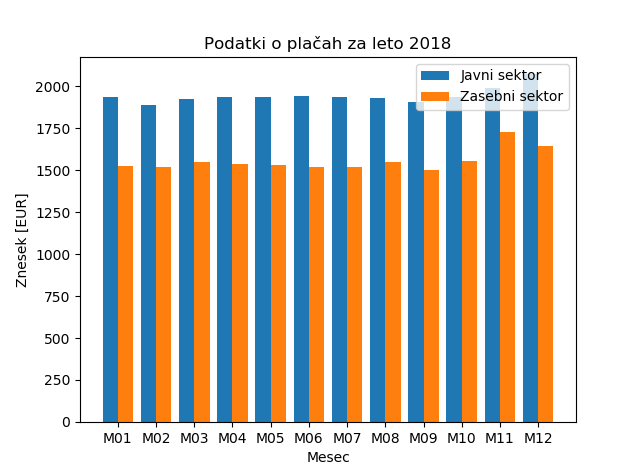
\includegraphics[width=\linewidth]{img/plt7.png}
    \caption{Dopolnjen in popravljen izris podatkov o plačah za leto 2018 s stolpčnim diagramom.}
    \label{img:plt7}
\end{figure}

\section{Risanje matematičnih funkcij}

Kaj pa če bi želeli narisati graf matematične funkcije? Podobno kot v zgornjih primerih, bomo funkciji za risanje podali seznam koordinat na osi $x$ in seznam koordinat na osi $y$. Koordinate na osi $x$ lahko določimo glede na željen razpon vrednosti -- tega določimo sami. Za določitev vrednosti na osi $y$ pa moramo funkcijo tabelirati pri podanih vrednostih osi $x$. Poskusimo na zgledu:

\begin{zgled}
Nariši grafe logaritemskih funkcij z osnovo 2, $\textrm{e}$ in 10 na intervalu od 0 do 5. Sliko opremi z legendami, vsak graf pa naj bo narisan s svojo barvo.
\end{zgled}

\begin{resitev}
Najprej bomo določili koordinate osi $x$. Lahko bi jih našteli, lahko pa uporabimo kakšno funkcijo za generiranje števil v podanem intervalu -- npr. funkcijo \texttt{range}.
\begin{lstlisting}[language=Python]
>>> X = range(6)
\end{lstlisting}
Če želimo v razpon vključiti tudi število 5, moramo kot argument \texttt{stop} podati število 6. Kako bomo prišli do funkcij za izračun logaritmov? Spomnimo se na modul \texttt{math}. Če pogledamo njegovo dokumentacijo, vidimo, da vsebuje funkcije \texttt{log2}, \texttt{log} in \texttt{log10}. Uvozimo jih. 
\begin{lstlisting}[language=Python]
>>> from math import log2, log, log10
\end{lstlisting}
Poskusimo zdaj izračunati koordinate točk na osi $y$:
\begin{lstlisting}[language=Python]
>>> Y_2 = log2(X)
TypeError: must be real number, not range
\end{lstlisting}
Tole ne bo šlo. funkcije za izračun logaritmov znajo delati samo s številskimi argumenti, mi pa smo podali seznam. Logaritem bomo morali torej izračunati za vsako točko posebej. Poskusimo najprej z dvojiškim logaritmom. Najprej bomo naredili prazen seznam. Potem bomo naredili sprehod čez vse točke na osi $x$ in za vsako posebej izračunali logaritem ter ga dodali v seznam.
\begin{lstlisting}[language=Python]
>>> Y_2 = []
>>> for x in X:
    Y_2.append(log2(x))
ValueError: math domain error
\end{lstlisting}
Kaj je narobe tokrat? Tokrat problem ni programerski, ampak matematični, saj logaritem števila 0 ni definiran. Razpon točk na osi $x$ bo torej potrebno zmanjšati na interval od vrednosti 1 do 5. Takole:
\begin{lstlisting}[language=Python]
>>> X = range(1,6)
>>> Y_2 = []
>>> for x in X:
    Y_2.append(log2(x))
\end{lstlisting}
Podobno naredimo še za naravni in desetiški logaritem in stvar narišemo. Celotna rešitev bo sledeča:
\begin{lstlisting}[language=Python,numbers=left,escapechar=~]
from math import log2, log, log10
import matplotlib.pyplot as plt

X = range(1,6) # koordinate točk na x osi

Y_2 = []
Y_e = []
Y_10 = []

for x in X:
    Y_2.append(log2(x)) # dvojiški
    Y_e.append(log(x)) # naravni
    Y_10.append(log10(x)) # desetiški

plt.plot(X,Y_2, label="$log_2(x)$")
plt.plot(X,Y_e, label="$log_e(x)$")
plt.plot(X,Y_10, label="$log_{10}(x)$")
plt.xlabel('x')
plt.ylabel('y')
plt.legend()

plt.show()
\end{lstlisting}
Graf, ki ga na ta način dobimo, prikazuje slika \ref{img:plt8}.\footnote{Oznake posameznih linij (\texttt{label}) smo podali med simboloma \texttt{\$}. S tem smo povedali, da podajamo zapis, ki ga bo Matplotlib pretvoril v enačbo. Zapis \texttt{\$log\_2(x)\$} bo Matplotlib tako izpisal kot $log_2(x)$. Pri takem načinu podajanja enačb moramo upoštevati pravila pisanja enačb v jeziku LaTeX, kjer je podčrtaj (\texttt{\_}) simbol za podpisan tekst.} 
\begin{figure}
    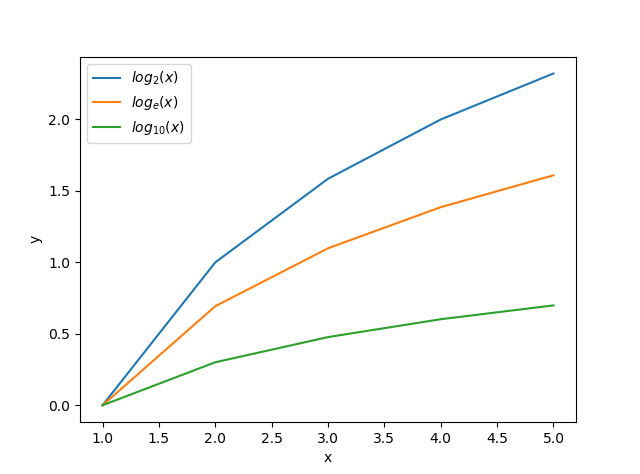
\includegraphics[width=\linewidth]{img/plt8.png}
    \caption{Osnovni izris logaritemskih funkcij.}
    \label{img:plt8}
\end{figure}
Problem je, da ta graf zgolj približno spominja na izris logaritemskih funkcij. Izrisali smo namreč samo 5 točk in te med seboj povezali. Prav tako nam manjka izris točk, ki imajo koordinato $x$ na intervalu (0, 1). Kako bi lahko \emph{resolucijo} izrisovanja povečali? Tako, da bi zmanjšali korak, s katerim generiramo koordinate na osi $x$. Idealno bi bilo, če bi izrisovanje začeli pri neki zelo majhni vrednosti $x$-a (npr. 0.001), potem pa to vrednost povečevali do števila 5, z nekim zelo majhnim korakom (npr. 0.001). Funkciji \texttt{range} bi to podali na sledeč način:
\begin{lstlisting}[language=Python]
>>> X = range(0.001, 5.001, 0.001)
TypeError: 'float' object cannot be interpreted as 
an integer
\end{lstlisting}
Problem tega pristopa je ta, da lahko funkciji \texttt{range} podamo samo celoštevilske argumente. Znajti se bomo morali torej drugače. Alternativen pristop bi bil, da s funkcijo \texttt{range} zgeneriramo točke od 1 do 5000, in potem vsako izmed njih delimo s 1000. Tako bomo dobili definicijsko območje z željeno resolucijo. 
\begin{lstlisting}[language=Python]
>>> X_cel = range(1,5001,1)
>>> X = []
>>> for x in X_cel:
	x /= 1000
	X.append(x)
\end{lstlisting}
Zdaj lahko pri računanju upoštevamo te vrednosti. Dopolnimo zgornjo kodo in poglejmo rezultat, ki ga prikazuje slika \ref{img:plt9}.
\begin{figure}
    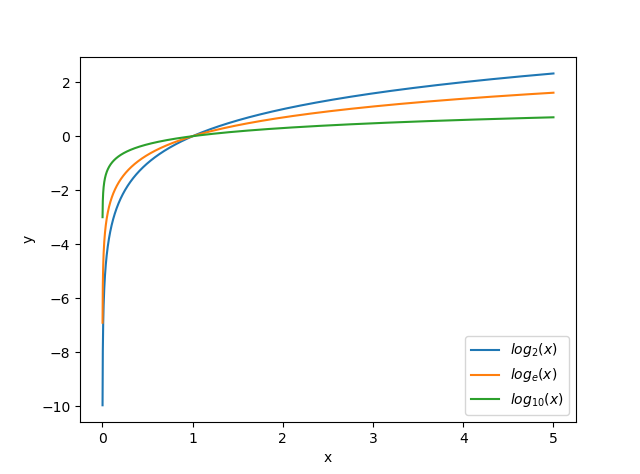
\includegraphics[width=\linewidth]{img/plt9.png}
    \caption{Izris logaritemskih funkcij z ustreznejšo resolucijo.}
    \label{img:plt9}
\end{figure}
Celotno rešitev prikazuje spodnja koda:
\begin{lstlisting}[language=Python]
>>> X = range(1,6)
>>> Y_2 = []
>>> for x in X:
    Y_2.append(log2(x))
\end{lstlisting}
Podobno naredimo še za naravni in desetiški logaritem in stvar narišemo. Celotna rešitev bo sledeča:
\begin{lstlisting}[language=Python,numbers=left]
from math import log2, log, log10
import matplotlib.pyplot as plt

X_cel = range(1,5001,1) # predpriprava za koordinate x

X = []
Y_2 = []
Y_e = []
Y_10 = []

for x in X_cel:
    x /= 1000 # koordinata x
    X.append(x)
    
    Y_2.append(log2(x)) # dvojšiki
    Y_e.append(log(x)) # naravni
    Y_10.append(log10(x)) # desetiški

plt.plot(X,Y_2, label="$log_2(x)$")
plt.plot(X,Y_e, label="$log_e(x)$")
plt.plot(X,Y_10, label="$log_{10}(x)$")
plt.xlabel('x')
plt.ylabel('y')
plt.legend()

plt.show()
\end{lstlisting}

\end{resitev}
Tole je bilo precej nerodno predvsem iz dveh razlogov. Prvič, za izračun logaritmov vseh vrednosti v seznamu \texttt{X} smo se morali sprehoditi čez cel seznam in vsako vrednost izračunati posebej. Veliko lažje bi bilo, če bi lahko funkcijo poklicali kar nad celotnim seznamom (brez uporabe zanke for). Drugič, funkciji \texttt{range} lahko podamo samo celoštevilske argumente. Ker smo želeli biti pri izrisovanju logaritmov nekoliko bolj natančni, smo morali generiranje definicijskega območja nekoliko zakomplicirati. Idealno pa bi bilo, če bi lahko funkciji \texttt{range} oziroma njej podobni funkciji podali decimalne korake. Izkaže se, da lahko zgornja problema rešimo z uporabo knjižnice \texttt{NumPy}, ki pa nam poleg tega olajša še marsikaj drugega.
